% 全等四判定 SSS/SAS/ASA/AAS 概览
\documentclass[tikz,border=4pt]{standalone}
\usepackage{ctex}
\usepackage{amsmath}
\usetikzlibrary{decorations.markings}
\begin{document}
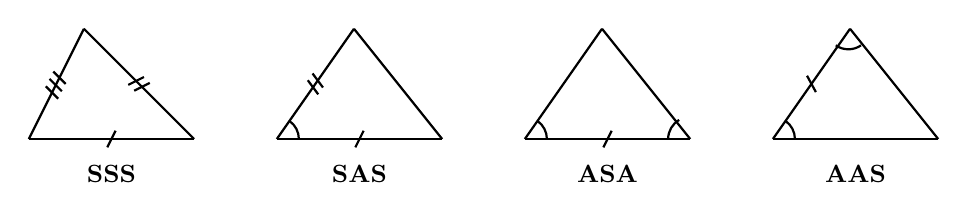
\begin{tikzpicture}[scale=0.7, thick,
  tick/.style={postaction={decorate, decoration={markings,
    mark=at position 0.5 with {\draw (-1.5pt,-3pt) -- (1.5pt,3pt);}}}},
  ticktwo/.style={postaction={decorate, decoration={markings,
    mark=at position 0.5 with {\draw (-2.5pt,-3pt) -- (-0.5pt,3pt);
                               \draw (0.5pt,-3pt)  -- (2.5pt,3pt);}}}},
  tickthree/.style={postaction={decorate, decoration={markings,
    mark=at position 0.5 with {\draw (-3.5pt,-3pt) -- (-1.5pt,3pt);
                               \draw (-0.5pt,-3pt) -- (1.5pt,3pt);
                               \draw (2.5pt,-3pt)  -- (4.5pt,3pt);}}}}]
  % SSS
  \begin{scope}[xshift=0cm]
    \draw[tick]      (0,0) -- (3,0);
    \draw[ticktwo]   (3,0) -- (1, 2);
    \draw[tickthree] (1,2) -- (0,0);
    \node[below] at (1.5, -0.3) {\small \textbf{SSS}};
  \end{scope}
  % SAS
  \begin{scope}[xshift=4.5cm]
    \draw[tick]    (0,0) -- (3,0);
    \draw[ticktwo] (0,0) -- (1.4, 2);
    \draw          (3,0) -- (1.4, 2);
    \draw (0.4,0) arc[start angle=0, end angle=55, radius=0.4];
    \node[below] at (1.5, -0.3) {\small \textbf{SAS}};
  \end{scope}
  % ASA
  \begin{scope}[xshift=9cm]
    \draw[tick] (0,0) -- (3,0);
    \draw (0,0) -- (1.4, 2);
    \draw (3,0) -- (1.4, 2);
    \draw (0.4,0) arc[start angle=0, end angle=55, radius=0.4];
    \draw (2.6,0) arc[start angle=180, end angle=120, radius=0.4];
    \node[below] at (1.5, -0.3) {\small \textbf{ASA}};
  \end{scope}
  % AAS
  \begin{scope}[xshift=13.5cm]
    \draw (0,0) -- (3,0);
    \draw[tick] (0,0) -- (1.4, 2);
    \draw       (3,0) -- (1.4, 2);
    \draw (0.4,0) arc[start angle=0, end angle=55, radius=0.4];
    \draw (1.6,1.7) arc[start angle=-55, end angle=-125, radius=0.4];
    \node[below] at (1.5, -0.3) {\small \textbf{AAS}};
  \end{scope}
\end{tikzpicture}
\end{document}
